
\documentclass[
    bachelor, 
    %bigskip, % sets linespread factor to 1.5
    propfont, % whether to use property fonts
    %nofont, % remember to manally set the fonts
    pdflinks,
    %colorlinks,
    %compact,
    ] {../base/xjtuthesis}

\usepackage[utf8]{inputenc}
\usepackage[T1]{fontenc}
\usepackage{graphicx}
\usepackage{listings}
\usepackage{xcolor}

\lstset{
    numbers=left,
    numberstyle= \tiny,
    keywordstyle= \color{brown},
    commentstyle= \color{gray},
    basicstyle=\footnotesize\ttfamily,
    frame=none,
    backgroundcolor=\color[rgb]{0.95,0.95,0.95},
    showstringspaces=false,
    xleftmargin=2em,xrightmargin=2em, aboveskip=1em,
    framexleftmargin=2em
}

\graphicspath{{figures/}}

\begin{document}

    
% 标题,中文
\ctitle{基于神经网络模型的人体姿态估计}

% 作者,中文
\cauthor{杜涵文}

% 学科,中文,本科生不需要
\csubject{}

% 学院,专业,班级,中文,本科毕业论文需要
\ccollege{电信}   % TODO 电信 or 计算机
\cmajor{计算机科学与技术}
\cclass{计算机少71}

% 设计所在单位,中文,本科毕业论文需要
\corgnization{西安交通大学}

% 学号
\stunum{2150506076}

% 导师姓名,中文
\csupervisor{魏平}

% 关键词,中文。用全角分号「;」分割
% 研究生的应首先从《汉语主题词表》中摘选
\ckeywords{人体姿态识别;动作捕捉;卷积神经网络;残差网络}

% 提交日期,本科生不需要
\cproddate{\the\year 年\the\month 月}

% 论文类型,中文,本科生不需要
% 从理论研究、应用基础、应用研究、研究报告、软件开发、设计报告、案例分析、调研报告、其它中选择
\ctype{}

% 论文标题,英文
\etitle{Human Pose Estimation Based on Deep Learning}

% 作者姓名,英文
\eauthor{Du Hanwen}
%todo 名字可能有错

% 学科,英文,本科生不需要
\esubject{}

% 导师姓名,英文
\esupervisor{Wei Ping}

% 关键词,英文。用半角分号和一个半角空格「; 」分割
\ekeywords{Human pose estimation; Motion capture; Convolutional neural networks; Residual networks}

% 学科门类,英文
% 从Philosophy(哲学)、Economics(经济学)、Law(法学)、Education(教育学)、Arts(文学)、
%   Science(理学)、Engineering Science(工学)、Medicine(医学)、Management Science(管理学)中选择 
\ecate{}

% 提交日期,英文,本科生不需要
% 应当和 cproddate 保持一致
\eproddate{\monthname{\month}\ \the\year}

% 论文类型,英文,本科生不需要
% 从Theoretical Research(理论研究)、Application Fundamentals(应用基础)、Applied Research(应用研究)、
%   Research Report(研究报告)、Software Development(软件开发)、Design Report(设计报告)、
%   Case Study(案例分析)、Investigation Report(调研报告)、其它(Other)中选择
\etype{}

% 摘要,中文。段间空行
\cabstract{

计算机视觉为人类社会工业界的重要支柱技术之一。随着深度学习的广泛应用,计算机视觉中人体姿态估计(HPE, human pose estimation)任务被注入了新的活力。同时随着基于摄像头的计算机视觉解决方案的广泛铺开,人体姿态估计在人机交互、游戏、虚拟现实、视频监控、运动分析、医疗辅助等领域有着广泛的应用。本文基于单目摄像头的视频采集,利用深度神经网络,完成了视频序列中单人的人体姿态估计任务,并有效地利用提取出的动作制作了人体模型三维动画。

人体姿态估计有诸多子课题,本文的工作主要聚焦在了单目单人RBG视频的三维人体姿态上。本文的工作选取了三维人体姿态估计中经典的两步提升思路,先将视频或图像中的人体关节点进行识别,预测出较为准确的二维坐标,再在此二维坐标结果的基础上预测出关节点的三维坐标。

在二维人体姿态估计上,采用了ResNet结构加以反卷积层,生成高分辨率的热力图以预测二维坐标。在三维人体姿态估计上,采用了一维空洞卷积网络处理视频序列间的时序信息,最终生成人体关节点的三维坐标序列。

最终,本文将人体姿态估计的实际应用场景定位在了动作捕捉三维角色动画生成上。利用上述的网络模型,针对日常的单人视频,提取出姿态序列。将其转换为动作捕捉记录文件类型后,对人体模型进行动作绑定,进而制作生动流畅还原度较高的三维角色动画。

}

% 摘要,英文。段间空行
\eabstract{

Computer vision is one of the important pillar technologies of human society industry. With the wide application of deep learning, the task of human pose estimation (HPE) in computer vision field has been injected with new vitality. At the same time, with the wide spread of camera-based computer vision solutions, human pose estimation has a wide range of applications in human-computer interaction, games, virtual reality, video surveillance, motion analysis, medical assistance and other fields. In this thesis, based on the video collection of monocular camera, the deep neural network is used to complete the single human body pose estimation task in the video sequence, and the 3D animation of human body model is made effectively by using the extracted actions.

There are many subjects of body pose estimation, and the work of this thesis mainly focuses on the 3D body pose of monocular single-person RBG video.The work of this thesis selects the classical two-step lifting idea in 3D body pose estimation. First, the body nodes in the video or image are identified to predict the more accurate 2D coordinates, and then the 3D coordinates of the nodes are predicted on the basis of the 2D coordinate results.

ResNet and deconvolution layer are used to estimate the 2D pose. Heat map is generated to predict the 2D coordinates. In 3D human pose estimation, a one-dimensional void convolutional network is used to process the time sequence information between video sequences, and finally generates the 3D coordinate sequence of human body nodes.

Finally, the actual application scene of human pose estimation is positioned in motion capture 3D character animation. Using the above network model, pose sequence is extracted for daily single person video. After converting it into motion capture record file type, action rigging is carried out on the human model to produce vivid 3D character animation.


}


    \xjtuchead
    \xjtucinfopage
    \xjtueinfopage
    \xjtutoc
    \clearpage

    % 主要符号表,可以没有
    %% denotation.tex
%
% Aetf <aetf@unlimitedcodeworks.xyz>
% Copyright 2016 Aetf <aetf@unlimitedcodeworks.xyz>
%
% multiple1902 <multiple1902@gmail.com>
% Copyright 2011~2012, multiple1902 (Weisi Dai)
%
% Project Home: https://github.com/Aetf/xjtuthesis
%
% It is strongly recommended that you read documentations located at
%   https://github.com/Aetf/xjtuthesis/wiki
% in advance of your compilation if you have not read them before.
%
% This work may be distributed and/or modified under the
% conditions of the LaTeX Project Public License, either version 1.3
% of this license or (at your option) any later version.
% The latest version of this license is in
%   http://www.latex-project.org/lppl.txt
% and version 1.3 or later is part of all distributions of LaTeX
% version 2005/12/01 or later.
%
% This work has the LPPL maintenance status `maintained'.
%
% The Current Maintainer of this work is Aetf.
%
\begin{denotation}

  \item[\xjtuthesis]    我能吞下玻璃而不伤身体噢
  \item[Linux]          李氏操作系统
  \item[Windows]        温氏操作系统

\end{denotation}


    \xjtucontent

        
\chapter{绪论}
\echapter{Preface}

视觉在是人类的重要感官之一,也是人类获取信息效率最高的感官,是人类认识和理解外界的重要途经,计算机视觉也相应成为了人类社会工业界的重要支柱技术之一。随着深度学习的广泛应用,计算机视觉在近年有了蓬勃的发展,人体姿态估计(HPE, Human Pose Estimation)任务也被注入了新的活力,有了越来越多的科研成果。同时随着基于摄像头的计算机视觉解决方案的广泛铺开,人体姿态估计也逐渐贴合了越来越多的实际场景,在人机交互、游戏、虚拟现实、视频监控、运动分析、医疗辅助等领域有着广泛的应用,是计算机视觉领域的热门研究课题。本文基于单目摄像头的视频采集,利用深度神经网络,完成了视频序列中单人的人体姿态估计任务,并有效地利用提取出的动作制作了人体模型三维动画。



\section{应用背景与意义}


人体姿态估计在实际应用中,为视频监控、行为分析、自动驾驶、虚拟现实、人机交互(HCI, Humancomputer interaction)、医疗辅助、游戏、电影和动画等多种场景提供了丰富的人体几何和运动信息。

例如在视频监控中,利用人体识别与人体姿态识别,可以实时监控楼宇、工地、社区等场所的高风险区域,发现攀高等危险行为时及时告警提醒,避免异常攀高导致安全事故;或对公共场所中人员突然奔跑或突然的人员聚集等情况进行检测和预判,助于安防疏导。在行为分析方面,如图\reg{fig:f1}所示,人体姿态识别可以辅助体育运动和训练中,对运动员或训练者的动作进行分析,分析其运动的习惯,辅助教练对不规范动作进行纠正等。在自动驾驶的研发中,需要对车辆行驶的路况进行分析和预测,此时需要对行人的朝向,姿态进行分析,进而预测可能的下一步行为,帮助车辆依此进行行驶决策。在人机交互中,如图\reg{fig:f2}所示,可以利用对人体动作的识别研发远程交互式体感游戏。

\begin{figure}[h!]
  \centering
  \subfloat[人体姿态估计辅助体育运动分析] {
      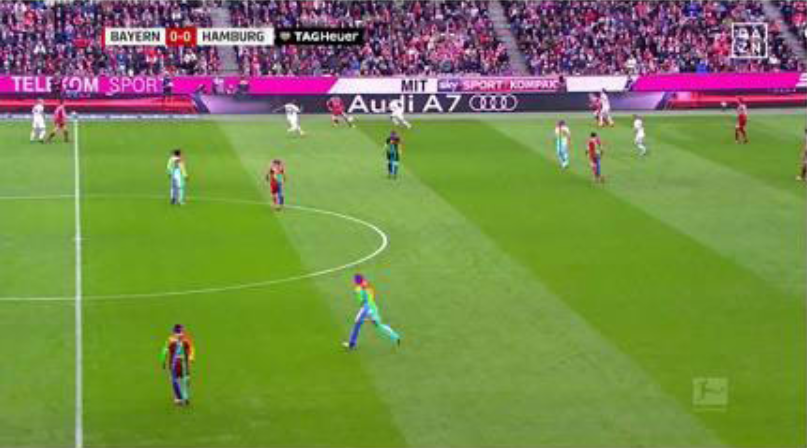
\includegraphics[width=6.67cm]{figures/1.png}
      \label{fig:f1}}
  \subfloat[基于人体姿态估计的体感游戏] {
      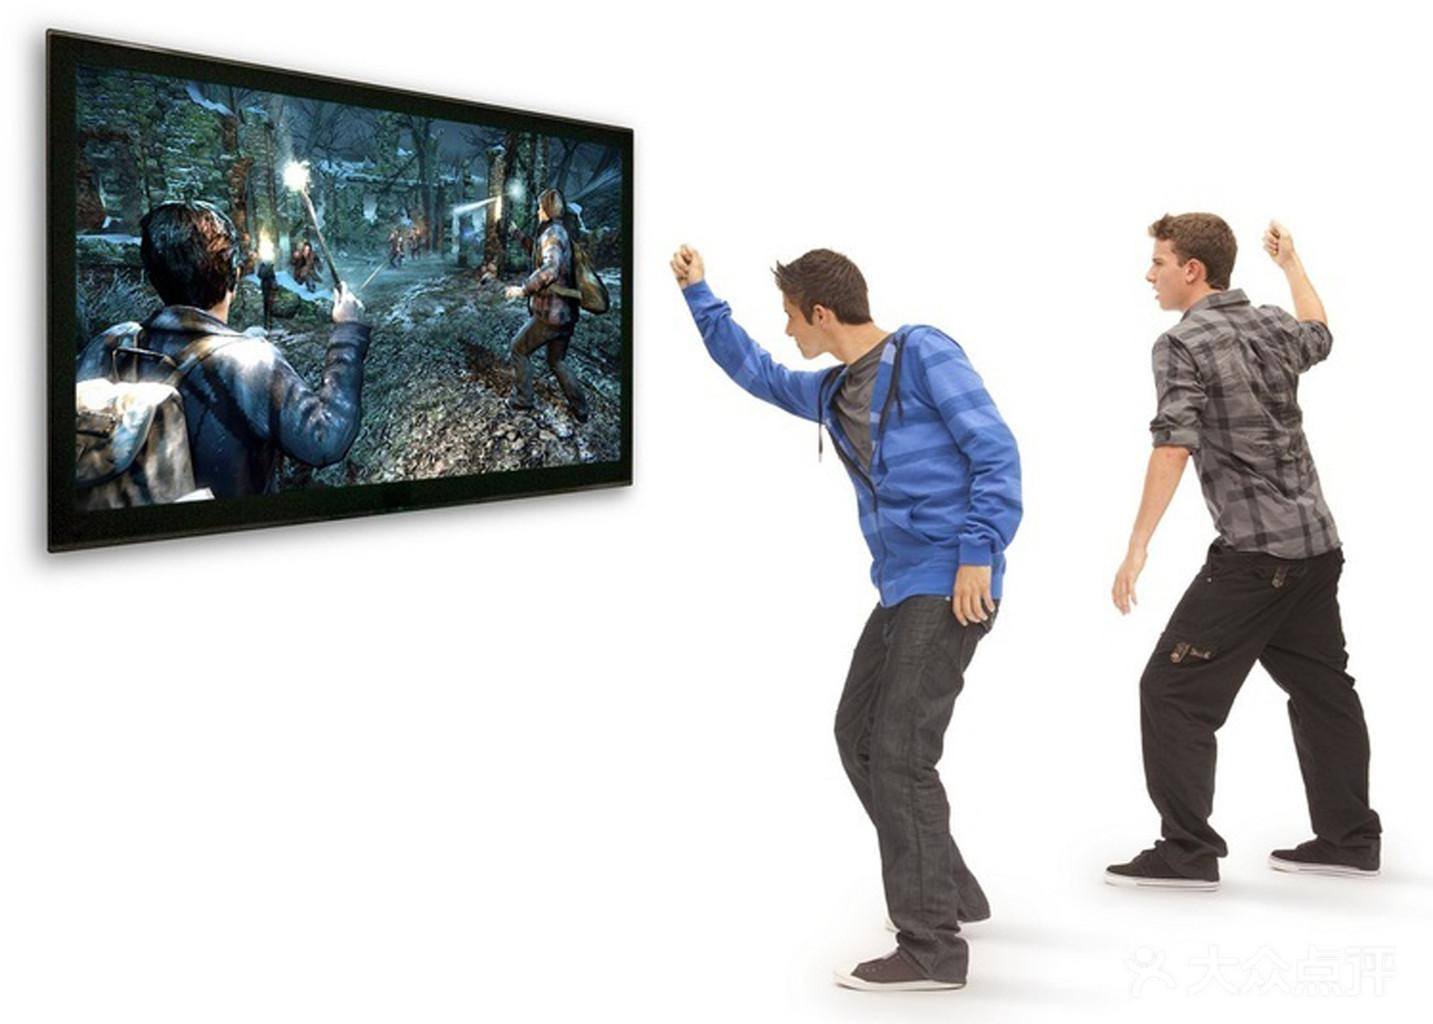
\includegraphics[width=6.67cm]{figures/2.png}
      \label{fig:f2}}
  \caption{人体姿态估计实际应用}
\end{figure}

人体姿态识别在近年来成为了人类社会各类产业中辅助生产的重要技术之一,本文的工作则将人体姿态识别应用在了影视动画创作领域,利用对视频中人体动作的分析,自动化生成具有相应动作的三维角色动画。

动作捕捉(MoCap, Motion Caption)是记录运动并在数字角色模型上创建运动的过程。动作捕捉可用于各种应用场景,例如运动,医疗应用,人体工程学,娱乐和机器人技术,以及三维角色动画,预可视化以及虚拟电影制作。更为具体地,当动作捕捉应用于游戏开发和电影制作中时,则主要指记录演员动作,来制作动画等具有视觉效果的媒体内容。

\begin{figure}[h]
	\centering
	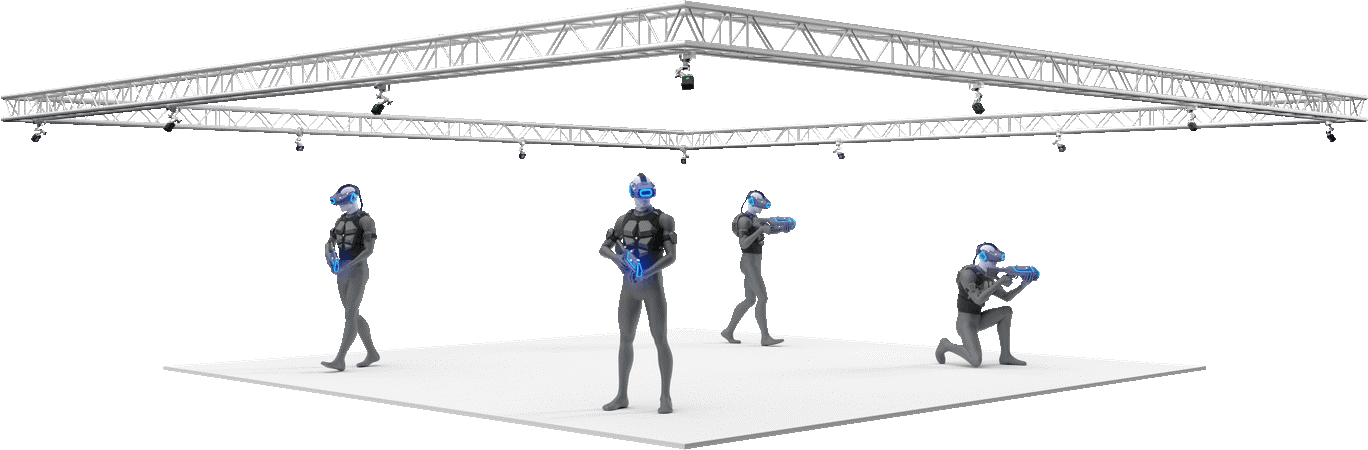
\includegraphics[scale=0.4]{figures/3.png}
	\caption{动作捕捉场地}
	\label{fig:f3}
\end{figure}

而这其中的主要动作捕捉技术主要依赖于硬件设备,从硬件设备的采集数据的原理上来说可以分为光学式、惯性式等。而除了一般动作捕捉系统中的穿戴式设备外、感应摄像头、符合光线要求的场地场所、相应软件以及基础的服务等对专业性的要求极高,价格不菲。根据相关调研报告,全球动作捕捉市场在2018年达到了1.632亿美元,并且预计到2026年,可以增长至2.617亿美元。同时预测复合年增长率在2019-2026年内为8.13%。

由于动作捕捉的价格昂贵,市场需求大,对动捕质量的要求随着动画产业的发展也在不断地增加。同时随着三维人体姿态估计的效果逐步提升,基于RGB摄像视频的动作捕捉成为了降低动画生成门槛的新的解决方案。



\section{课题主要任务}{}

人体姿态估计指在从图像或视频中,对任务目标的姿态进行识别和估计。

输入数据一般为采集的RGB图像或RGB-D图像,可以为单目单视角(Monocular)图像或使用多个摄像机针对相同的目标同一时刻的动作进行采集的多目多视角(Multi-view)图像,图像中可以包含一个人体目标或多个人体目标。

首先通过人体识别获得每个目标人体所在的区域或边框(bounding box),进一步通过热力图(heatmap)

对人体的各个关键点位置进行概览预测或直接回归出各关键点的坐标。可以通过对头部、颈部、髋部、膝盖等人体的重要关节点进行坐标预测来描述人体骨架,或通过估计出符合人体形状的蒙皮描述人体的姿态,例如图\reg{fig:f4}右侧蒙皮图像所示,SMPL模型(Skinned Multi-Person Linear (SMPL) Model),便利用具有10个维度的形状参数和描述24个关节点的姿态参数描述整个人体的蒙皮。

\begin{figure}[h]
	\centering
	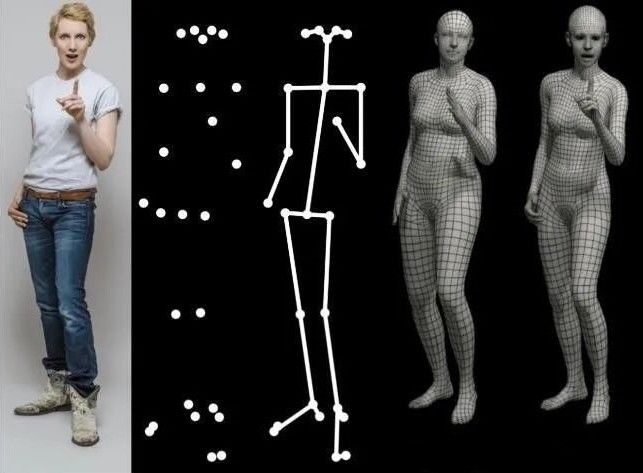
\includegraphics[scale=0.4]{figures/4.jpg}
	\caption{人体姿态描述模型}
	\label{fig:f4}
\end{figure}

此外,可以仅针对单帧图像进行估计,也可以在视频中,针对帧序列中的人体进行姿态序列的分析。在对帧序列进行姿态估计时,需要对同一个目标人物进行追踪,并利用时序模型来提取上下文信息,估计出准确连贯的姿态序列。

最为主要地,根据输出的数据维度,也即描述人体姿态关节点的坐标维度,可以划分为二维人体姿态估计与三维人体姿态估计两大部分。二维人体姿态估计的目标是定位图像中每个关键点的(x,y)坐标,而三维人体姿态估计的目标是推断三维空间中每个关键点的(x,y,z)坐标。

本文的工作主要集中在了对单目单人RGB视频中的目标进行姿态估计。基于此类数据的人体关节点坐标的恢复具有其独特的特征和挑战,其挑战主要在于三点:

其一,柔性体构型意味着复杂的相互依赖的关节和高自由度的肢体,这可能会导致出现自遮挡及其他罕见且复杂的姿态。

其二,是人体呈现的多样性,包括服装的多样及自身极为相似的部位。

其三,复杂的拍摄环境常导致前景的遮挡,加之多样的拍摄角度和画幅的不完整,导致目标与周围人的相似部位出现混淆。



\section{国内外研究现状}

\subsection{二维人体姿态估计}{}

早期的二维人体姿态估计融入了许多特征的构建,比如描述运动信息的梯度方向直方图(HOG, Histogram of Oriented Gradient)和小边特征(Edgelet)
等,但这些方法在实践中并不具备精确估计的能力。随着深度神经网络的发展,深度学习方法则更能够从元数据重提取出更充分的特征,产生了优异的结果,并在很大程度上超过了传统方法。基于方法分类的二维人体姿态估计任务如图\reg{fig:f5}。

\begin{figure}[h]
	\centering
	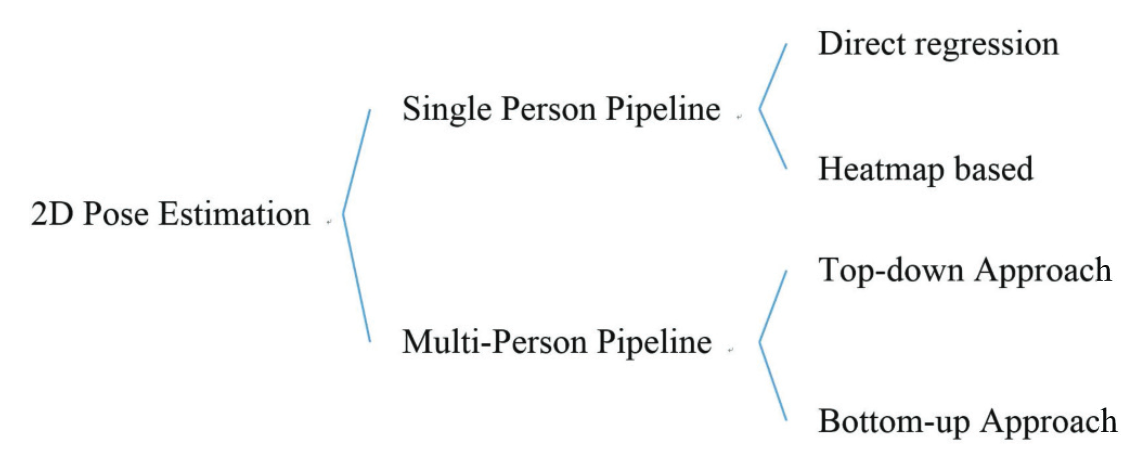
\includegraphics[scale=0.4]{figures/5.png}
	\caption{二维人体姿态估计分类}
	\label{fig:f5}
\end{figure}

单人姿态估计从预测关键点的方法上主要分为直接回归方法与热力图方法两类。前者利用输出特征映射直接回归关键点,如facebook于2018年搭建的DensePose。后者则首先生成热图(heatmap),用其中的像素值表示关键点在该位置存在的概率,并根据热图预测关键点,如2016年的Hourglass。

而多人姿态估计的整体思路主要分为两类。第一种为自顶向下的方法,指的是首先从全图的范围上进行人体检测,然后切入到每个目标人体的范围,进行单人关键点估计,如2016年提出的AlphaPose。自底向上的方法的第一步则是定位图像中的所有关节点,第二步是将关节点向上分组为人体,2016年提出利局部关联域(PAF, Part Affinity Field)方法进行关键点组装的OpenPose。

\subsection{三维人体姿态估计}{}
三维人体姿态估计相对于二维人体姿态估计具有更多难点,其一是单目图像及视频信息本身具有的歧义性,即一个二维的姿态投影可以对应多种三维的姿态。其二是需要利用昂贵的设备和严苛的环境条件进行三维姿态数据集的采集较为困难,故而对网络的泛化性要求也更为严格。

\begin{figure}[h]
	\centering
	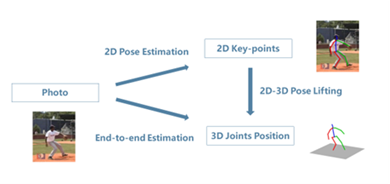
\includegraphics[scale=0.4]{figures/6.png}
	\caption{三维人体姿态估计两大思路}
	\label{fig:f6}
\end{figure}

如图\reg{fig:f6}所示,基于深度学习的三维人体姿态估计方法可主要分为两大思路。第一种思路为两步式,先从图像中提取出二维关节点坐标,再将其从二维提升到三维坐标,如Facebook AI于2018年提出的VideoPose三维模型。第二种思路为端到端式,从视频和图像中直接回归出三维坐标,如Li等于2014年利用卷积神经网络搭建的包括关节检测与坐标回归两支路模型。此外,还有工作选择融合式模型,在两步式的第二步估计过程中仍然融入源数据。

\subsection{视频动作捕捉}{}
无硬件设备需求的视频人体动作捕捉解决方案提供商在近几年,于国内外如雨后春笋般崛起并在持续地发展。

如国内云舶提供的对单人视频进行捕捉的小K动捕,对人物的脚-地接触进行了优化,使其接触稳定,无垂直的浮动。此外,美国DeepMotion也提供了包含单人动作捕捉以及人物追踪等多种视频解决方案。同时,Ridical也提供了粒度细至手指关节的实时视频动作捕捉API。

\begin{figure}[h]
	\centering
	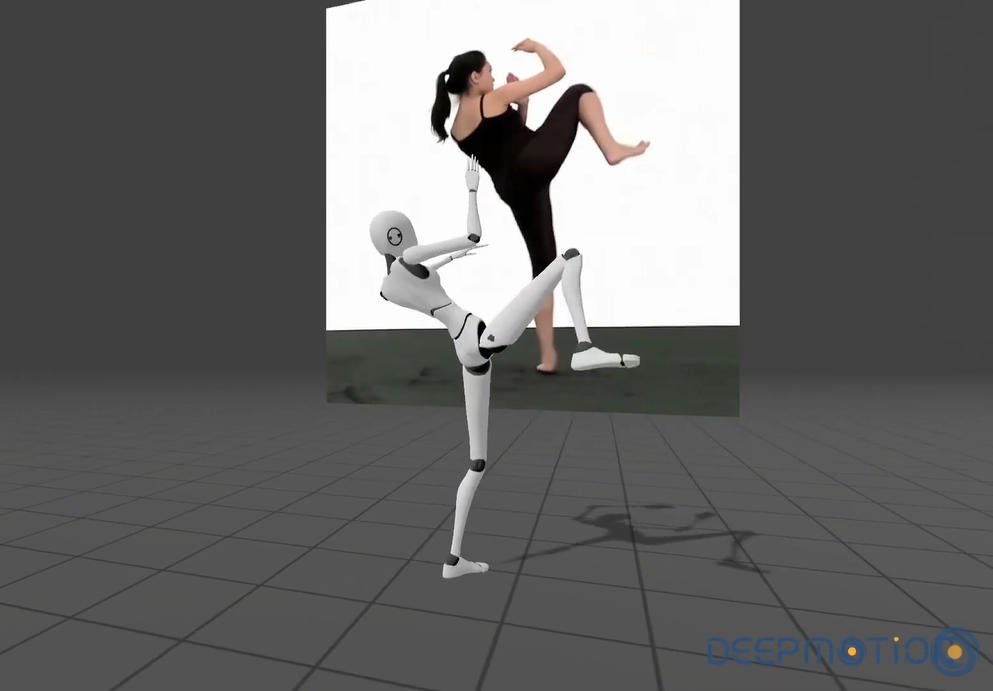
\includegraphics[scale=0.4]{figures/7.png}
	\caption{DeepMotion视频动作捕捉}
	\label{fig:f7}
\end{figure}



\section{本文主要工作内容}


\subsection{本文工作}{}
针对人体姿态估计任务,本文的工作主要聚焦到了基于深度神经网络模型,对日常场景中,单目RGB摄像头采集的单人动作视频进行姿态估计,并利用估计出的人物动作制作三维角色动画。整体流程首先输入单人视频,利用残差网络搭建二维关节点估计模型,并利用一维空洞卷积提取视频中的时序信息,将二维关节点坐标提升为三维坐标,最后将三维坐标转换为描述动作文件的人体骨架欧拉角,进行三维角色绑定。

\subsection{论文结构安排}{}
本文共包含六个章节,各章节的具体内容概括如下。

第一章:绪论。在绪论中,首先介绍了人体姿态估计课题的研究意义以及在各实际领域的应用价值,尤其是在动作捕捉领域,具有旷阔的市场和可期的前景。接着介绍了人体姿态估计的任务的具体目标及当前工作的研究现状。最后对本文的主要工作进行了简要的概括 ,并对本文的章节安排进行了介绍。

第二章:人体姿态识别相关基础。在第二章中,针对计算机视觉尤其是人体姿态估计中常用到的经典的深度学习模型及方法进行了介绍,包括卷积神经网络、残差网络等,它们构成了第三章及第四章模型的基础架构。同时介绍了人体姿态描述模型与动作捕捉相关设备与数据文件。

第三章:基于反卷积神经网络的二维人体姿态估计。本章重点说明了用于二维人体姿态估计的模型,一个相对于之前的Hourglass和CPN结构都更为简单明了的网络结构。模型利用热力图对人体关节进行二维坐标的预测,并在网络中利用反卷积进行上采样,用以得到高分辨率的特征图。

第四章:基于空洞卷积神经网络的三维人体姿态序列估计。本章首先针对三维人体姿态估计任务的主要问题进行了分析,并采用了二步提升法,同时利用卷积神经网络处理视频中的时序信息,进行三维人体姿态的估计。

第五章:视频动作捕捉动画生成。在本章中,利用第三章及第四章的网络模型所预测出的人体姿态,对人物角色模型进行动画生成。搭建了人体骨骼模型,将关节点坐标转换为了动作描述文件bvh所需的欧拉角。并在MotionBuilder软件中对人物模型进行了动作绑定,制作出了还原度极高且稳定的三维动画。

第六章:总结与展望。本章归纳和总结了本文针对人体姿态估计任务所做的工作,以及针对视频动作捕捉进行的工程搭建。对人体姿态估计的后续研究方向以及视频动作捕捉的未来进行了更深层次的探讨和展望。





        
\chapter{人体姿态估计相关基础}
\echapter{Preface}


\section{深度学习基础}


机器学习(ML, Machine Learning)中深度学习(DL, Deep Learning)领域,是近几年蓬勃发展,在诸多场景下都大放异彩的一大研究方向,随着可用于学习的数据的增加,算力的增强以及视觉传感器的研发,深度学习在计算机视觉方面有着广泛的应用和优秀的表现。本节将针对深度学习发展到近年,构成深度学习基础的诸多经典模型及方法进行精炼的介绍。



\subsection{卷积神经网络}{}

1989年,LeCun提出的一种基于卷积运算神经网络,卷积神经网络(CNN, Convolutional neural network),现常用于在深度学习中对图像任务进行处理。

在卷积网络应用之前,神经网络的架构基本为全连接层,对于图像信息,全连接层网络的参数十分庞大,特征提取效率低,训练时间长。而卷积神经网络通过稀疏连接,构建较小的感受野并共享参数,加以卷积计算,相比于传统神经网络大大降低了网络的复杂度,减少了计算量,使得网络的深度得以增加。

同时,卷积神经网络最突出的特征就是能够尽可能地自动拟合所需要的特征。与其他图像分类算法相比,卷积神经网络对输入的数据格式要求极为简单,所需要的预处理较少,这意味着网络将更多地通过自动学习各种特征来优化卷积核。相对于传统的机器学习以及全连接网络等需要手工处理特征的模型,这种不依赖于先验知识和人工干预的特征提取是一个重要的优势,可以尽可能地保留原始信息,挖掘潜在规律。

此外,卷积神经网络对于具有网格状拓扑(如图像)的数据非常理想,因为在卷积和池化过程中,单独特征之间的空间关系也被加以提取。

在已有的工作中,可以看到这种特征提取可以拟合出人类对图像的直观理解。人类的视觉感知主要强调对物体的样例变化,几何变换,背景变化等线性与非线性的变化,这些强大的认知能力由视觉神经系统支持。而卷积神经网络,受猫的视觉神经结构启发而构造,可以模拟人类视觉神经,首先感知到色彩、亮度、对比度,再到边缘,角点等细节特征,更深层次可以提取出纹理,形状等复杂信息和特征,模拟的视觉低、中、高维的认知便由这些特征复合组成。

卷积神经网络的隐藏层通常由两部分组成,第一部分为线性变换部分,包括卷积层、池化层和全连接层等,第二部分为非线性变换部分,如激活函数。本质上,卷积神经网络可以视为一个连续的线性加权滤波器接以非线性函数。

卷积神经网络的输入是一个张量,可以处理多维数据。卷积层由一组可学习的卷积核构成,每个卷积核对应一个范围较小,取决于卷积核大小的感受野。组成卷积核的每个元素都对应一个权重系数和一个偏移量,是进行特征提取的主要结构。卷积核会扫过输入的多维数据,并依次对每块感受野进行卷积操作,将结果输入至下一层。卷积操作即卷积核对感受野内的输入数据做矩阵元素乘法求和并叠加偏移量。

\begin{figure}[h]
	\centering
	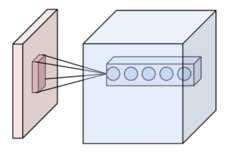
\includegraphics[scale=1.2]{figures/8.png}
	\caption{卷积核感受野及其输入和输出}
	\label{fig:f8}
\end{figure}
经过卷积层后,图像被抽象为新的形状和维度的特征图,通常被送进池化层进行池化操作,起到非线性降采样的作用。在保证平移不变性、尺度不变性等情况下,对图像不同位置的特征聚合统计,对卷积层输出的特征映射进行筛选过滤,压缩参数量,精简计算过程。一般所用到的池化方法有最大值池化和平均池化。池化层不需要学习参数,仅需要指定池化类型,池化操作核的大小和池化操作的步长即可。最大值池化每次操作时指定窗口大小,保留每个窗口中最大的数值,分别作用于输入特征图的各个通道,通道之间 不会相互影响;平均池化是对邻域内特征点取平均。池化层的引入降低特征图的计算量,并具有一定的平移不变性,在整个过程中不会丢失重要信息,一定程度上可以降低网络模型训练时过拟合的概率,提升神经网络的泛化能力。在卷积神经网络架构中,通常会在连续的卷积层(每个卷积层后面通常跟着一个激活函数,比如ReLU层)之间周期性地插入一个池化层。

此外卷积神经网络在训练的过程中,随着层层的提取,数据的分布会不断地变化并加以积累。故而在通常在网络中加以批归一化层来抑制中间层数据分布发生变化的情况。同时有效避免了网络收敛速度慢,梯度爆炸等情况,加速模型训练。

通常在卷积神经网络的最后会加以全连接层实现最终的分类等任务。可以将整个模型理解为通过层层全连接和池化层将原视信息映射到了一个隐空间,并通常由全连接层将特征映射到样本标签空间。

2012年Hinton等提出的AlexNet,以及2014年的VGG等便为经典的卷积神经网络模型。



\subsection{残差网络}{}

在2012年左的图像相关竞赛中,越来越深的神经网络模型依次展现了最好的表现。在网络层数的逐步加深时,深度残差网络可以说是近几年来计算机视觉及深度学习领域最具开创性的工作。残差结构使得网络可以训练到数百层且仍然具有较好的性能。
在图像相关的场景下,更深的网络意味着具有提取更多特征的可能性,故而堆叠越来越深的网络成为了一大趋势,用来丰富特征的维度。在网络层数的加深过程中时,虽然在一些场景下网络表现出了更高的精度和准确性,但也常常伴随着一些问题。例如梯度消失(Gradient Vanishing)和梯度爆炸(Gradient Exploding)。
当采用基于梯度的学习方法和反向传播来训练神经网络的时候,每一个神经网络的权值在每次训练迭代中接收一个与误差函数相对于当前权值的偏导数成比例的更新,此时浅层的偏导即为多个很小的偏导的乘积。当网络加深时,浅层的网络梯度便接近于0。而当梯度很小时,网络的学习速度极低,甚至完全阻止神经网络进行进一步的训练。如果该层网络的梯度一直很小,无法得到充分的训练,该层对整个网络便几乎不做贡献。类似地,当使用导数可以取较大值的激活函数时,则更易遇到爆炸梯度问题。
事实上,如图\ref{fig:f9}所示,实验表明,在进行传统的深度学习的训练过程中,随着ImageNet模型的网络层数的增加,最初越来越深的浅层网络的表现也越来越好,但当网络加深到一定阈值后,其准确率出现了退化(Degradation),训练误差越来越大。

\begin{figure}[h]
	\centering
	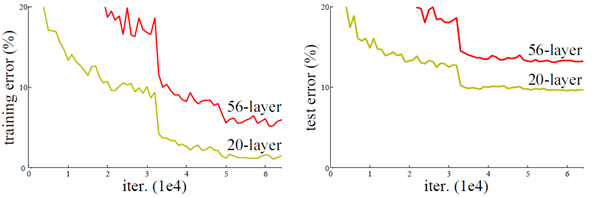
\includegraphics[scale=1]{figures/9.png}
	\caption{20层与56层的ImageNet网络误差}
	\label{fig:f9}
\end{figure}

解决梯度消失问题最有效的方法之一便是He等于2016年提出的残差神经网络,构建了跳跃连接来创建信息的“高速公路”,允许梯度信息通过各个层。其中前一层的输出被添加到更深一层的输出,这使得来自网络早期部分的信息可以被传递到网络的更深层部分,从而帮助在更深的网络中维持信号传播,对深层的网络重新引入浅层的输出来补偿消失的数据,同时解决了网络加深时的退化问题。
图\ref{fig:f10}为一个残差学习单元 (Residual Block),由两部分组成,右侧曲线为跳层连接的直接映射部分(Shortcut Connection),左侧曲线则包含卷积部分。

\begin{figure}[h]
	\centering
	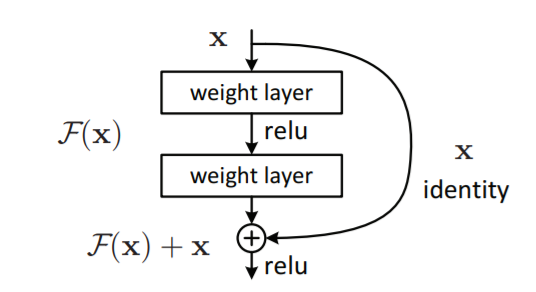
\includegraphics[scale=0.4]{figures/10.png}
	\caption{残差模块}
	\label{fig:f10}
\end{figure}

随着ResNet在研究领域的日益普及,其体系结构也得到了越来越多的研究,构造了许多基于ResNet的新体系结构。如Xie等人提出的一种ResNet的变体ResNeXt,其构建模块如图\ref{fig:f11}。

\begin{figure}[h]
	\centering
	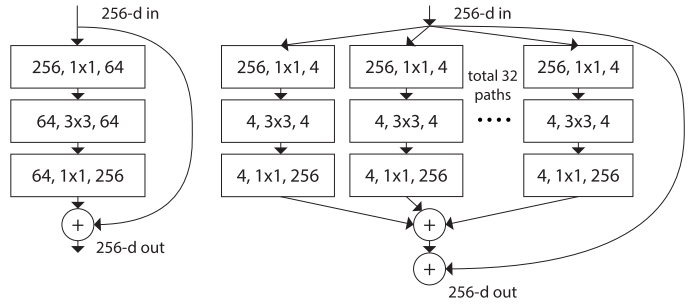
\includegraphics[scale=1]{figures/11.png}
	\caption{ResNeXt基本单元样例}
	\label{fig:f11}
\end{figure}

除此之外,Huang等人提出了一种名为DenseNet的新型架构。在ResNet中,跳跃连接主要是将距离较近的网络层之间进行连接,并让残差块串联组成整个网络来避免梯度消失和梯度爆炸以及网络的退化。DenseNet进一步利用了跳跃连接的效果,它使用跳跃连接,将所有神经网络层直接连接在一起。也就是说,对于每一层来说,其要处理的输入数据由在此之前全部的更浅层的特征图组成,其输出被传递到每个后续层。除了解决梯度消失的问题,这种架构同时支持了特性重用,使网络的参数效率大大提高。



\section{人体姿态描述模型}
本文的工作采用人体关节点坐标来描述人体的姿态。在human3.6m数据集中,人体关节点定义及编码如图\ref{fig:f12}所示:
0-Hip, 1-RightHip, 2-RightKnee, 3-RightAnkle, 4-RightSole, 5-RightToe, 6-LeftHip, 7-LeftKnee, 8-LeftAnkle, 9-LeftSole, 10-LeftToe, 11-Hip’, 12-Chest, 13-Neck, 14-Chin, 15-Head, 16-Neck’, 17-LeftShoulder, 18-LeftElbow, 19-LeftWrist, 20-LeftWrist’, 21-LeftOuterThigh, 22-LeftHand, 23-LeftHand’, 24-Neck’, 25-RightShoulder, 26-RightElbow, 27-RightWrist, 28-RightWrist’, 29-RightOuterThigh, 30-RightHand, 31-RightHand’

\begin{figure}[h]
	\centering
	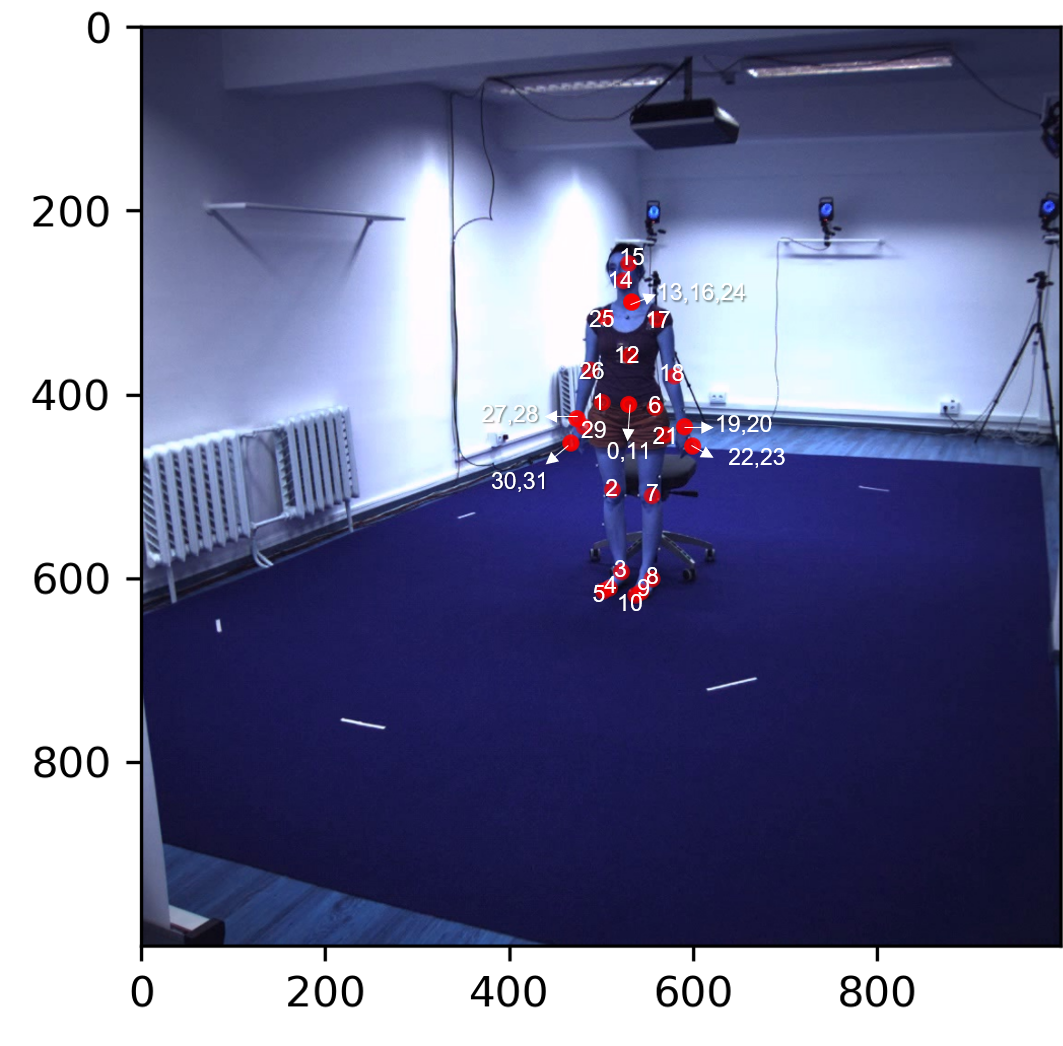
\includegraphics[scale=0.4]{figures/12.png}
	\caption{Human3.6m人体关节点标签及编码}
	\label{fig:f12}
\end{figure}


\section{动作捕捉}

\subsection{动作捕捉设备}{}
动作捕捉设备是运动物体的关键部位设置跟踪器。根据其技术原理分为惯性式、光感式等。并且由传感器、信号捕捉设备、数据传输设备与数据处理设备组成。
三维人体姿态数据的采集所需的动捕系统较为复杂,采集的数据格式与形式多样,以Human3.6m三维人体姿态数据集的采集系统为例。如图x所示,有4个数码摄像机,1个ToF时间飞行传感器和10 个动作捕捉相机共15个传感器。理论捕获区域大约为 6m x 5m,有效捕获区域大约 4m x 3m,在其中的对象对所有视频摄像机完全可见。
一组 10 个动作捕捉 (MX) 摄像机安装在墙壁上以最大化有效实验区域,左右边缘各 4 个,底部水平边缘大致中间 2 个。同时,还利用了Human Solutions (Vitus Smart LC3) 3D 激光人体扫描仪用于为参与实验的每个主体演员获得准确的 3D体积模型。
\begin{figure}[h]
	\centering
	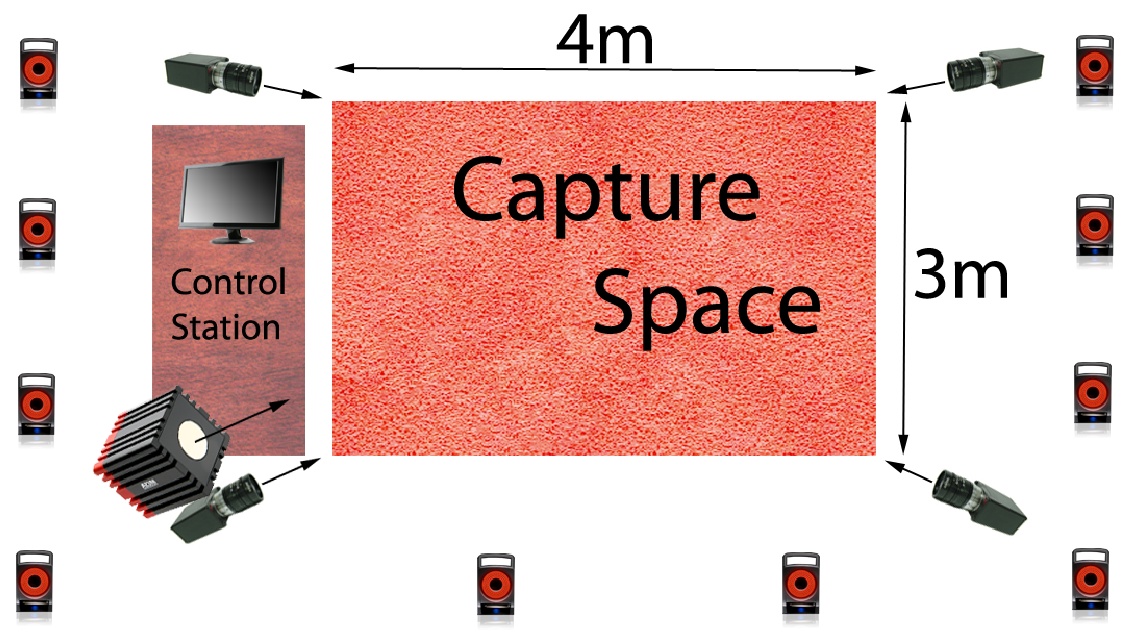
\includegraphics[scale=0.4]{figures/13.png}
	\caption{Human3.6m数据集采集区域}
	\label{fig:f13}
\end{figure}
数据集对以上各传感器的数据进行处理后,提供了各个相机的图像坐标系中的二维人体关节点坐标,三维人体关节点坐标,人体关节角度及人体三维扫描模型等。
而更为日常地,在普通的轻量级动作捕捉需求上,常见的惯性动作捕捉设备所采集的数据为bvh(Biovision hierarchical)文件格式,仅记录了相应的人体骨架中各个骨骼或关节点的相对旋转角度。
\begin{figure}[h]
	\centering
	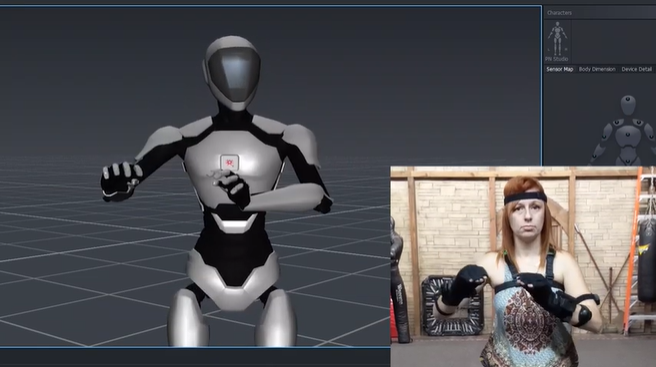
\includegraphics[scale=0.4]{figures/14.png}
	\caption{惯性动作捕捉设备及模型绑定效果}
	\label{fig:f14}
\end{figure}


\subsection{动作捕捉数据文件}{}
bvh(Biovision hierarchical data)是BioVision等动作捕捉设备对人体运动进行捕获后产生文件格式的文件扩展名,同时可用于对其他角色骨的动作描述,如机器狗等。bvh文件主要记录了角色的骨骼树和其中的肢体关节在各帧中的旋转数据来描述运动。bvh 文件已经成为了一种通用的角色特征动画文件格式,MotionBuilder、3DMax等动画生成软件皆支持bvh文件的导入和编辑。
bvh文件由两部分组成,头部信息和之后的数据部分。bvh文件如图\ref{fig:f15}所示,头部信息首先包含了目标物体的各个关节点及其继承关系,同时包括了描述关节点运动的旋转和位移两种通道,以及默认骨骼模型中各个关节点相对于父节点的局部偏移量。最后,头部信息中还包含了文件描述的动作的帧数以及每帧时长,默认单位为秒。在bvh文件的数据部分,从第一帧开始,以深度优先遍历骨骼树的顺序依次对每个关节点的各个数据通道进行记录,直到最后一帧。
\begin{figure}[h]
	\centering
	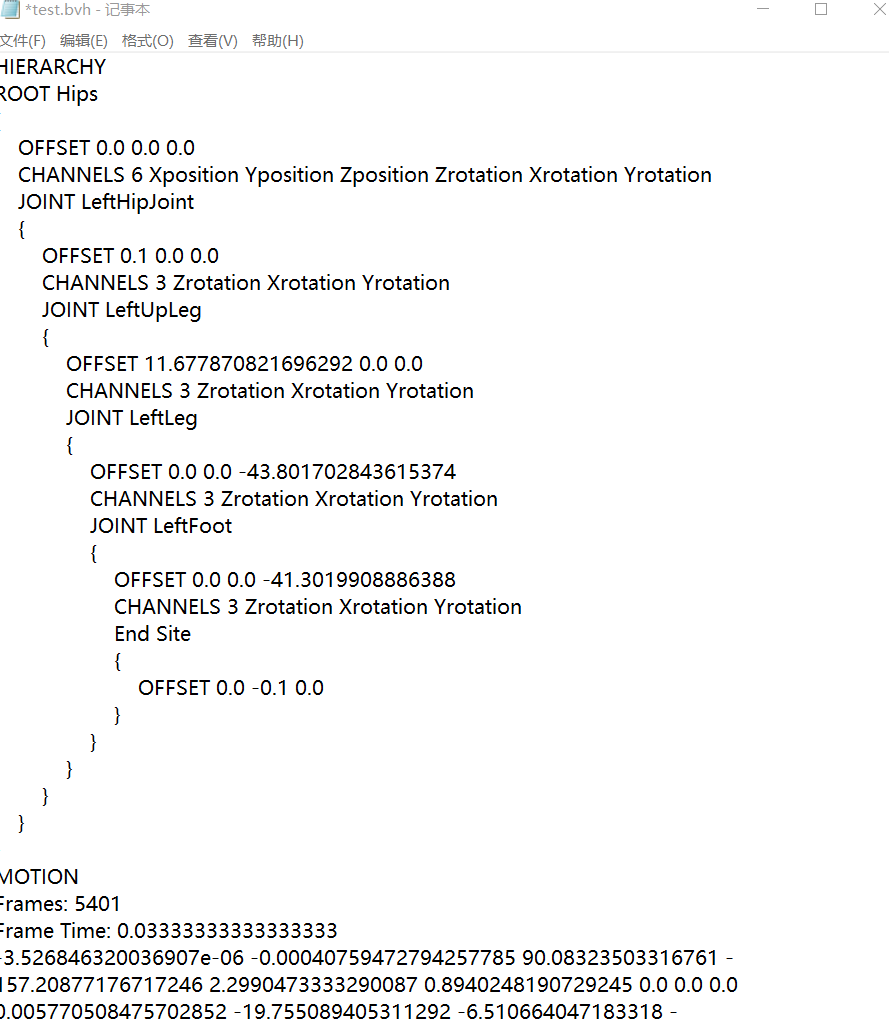
\includegraphics[scale=0.4]{figures/15.png}
	\caption{bvh文件样例}
	\label{fig:f15}
\end{figure}
关节树唯一的根节点关节,JOINT指所有的子关节,OFFSET记录子关节相对于父关节的偏移量,CHANNELS表明数据记录部分对应的各个通道。特殊地,ROOT关节的通道中必须包含Xposition、Yposition、Zposition三个位移信息,而子节点的位移信息在具有rotation信息时为冗余数据,可以省略。

\subsection{欧拉角}{}
刚体运动(rigid motion)由旋转(rotation)和平移(translation)两部分组成,在描述人体的运动时,可以将人体抽象为由关节点组成的骨架,并将骨骼的运动近似为刚体运动。
对于已知的一次旋转变换,通常可以用旋转矩阵(Rotation matrix)来表示。
而由于旋转矩阵有九个量,所以用它来描述只有三个自由度的一次旋转是冗余的。同时考虑到旋转矩阵具有行列式为1的正交矩阵的约束,使得后续针对旋转矩阵的估计和优化较为困难。故而本文选择更为直观和简洁的欧拉角来对骨骼的旋转运动进行最终的描述和记录。
欧拉角的基本原理是记录目标绕一个轴旋转的角度,并将一次旋转分解为三次绕不同的轴的旋转,并规定绕三个轴旋转的次序以及旋转轴在之前的旋转中的固定与否。最终,欧拉角描述旋转的形态为一个三维向量。
通常,在欧拉角的描述过程中,利用了两个坐标系,固定不动的世界坐标系xyz与随着物体的旋转而动的局部坐标系xyz。初始情况下,欧拉角描述的第一个旋转轴与世界坐标系的一个坐标轴一致。
假设局部坐标系与世界坐标系所形成的方向余弦矩阵(DCM, direction cosine matrix)已知,可得欧拉角如下。其中旋转顺序为Z-Y-X,物体先绕z轴旋转偏航角(yaw)的角度,再旋转之后的绕y轴旋转俯仰角(pitch),最后绕旋转之后的x轴旋转滚转角(roll)。

        
\chapter{基于反卷积神经网络的二维人体姿态估计}
\echapter{Preface}


\section{问题分析}
\esection{}
二维人体姿态估计具有如下难点:

\begin{enumerate}
    \item 遮挡和自遮挡。在复杂环境下和多人图像中,目标人体的部位难以避免地被前景、他人和自身部位及衣着遮挡,故而产生难以检测的关节点。
    \item 复杂的前景背景。除了遮挡之外,在多人姿态估计中,相邻目标人体的相似部位易导致区分和还原每个目标的正确姿态时发生混淆。
    \item 多样的人体姿态。除了人体的常见动作,如由走、坐构成的日常行为外,在极端的场景和特殊的相机视角下,会出现很多罕见的二维姿态投影,而难以被数据集覆盖。
\end{enumerate}

在训练中,为了加速卷积神经网络的训练,热图能够提供更多的监督信息,而不仅仅是关节点坐标。如图x所示,每个关节占据一个以目标关节位置为中心的二维高斯分布的热图通道。热图表示比坐标表示具有更强的鲁棒性,最近的研究大多基于热图表示。

同时,在对RGB图像进行关节坐标的预测时,对关节点进行精确的识别和坐标预测需要局部的细节信息,同时估计整个人体合理的姿态又需要对全局信息有正确的把握,以获取如人物朝向,肢体方位关系等信息。故而在网络架构中,进行下采样后,再上采样生成高分辨率特征图成为了网络设计的关键技术。

针对如上问题所涉及的网络架构越来越复杂,在进行算法分析时的对照也愈加苦难,无法针对算法中的每一个细节设计进行细致准确且严谨的分析。故而本文希望在同时准确传局部信息和全局信息的同时构建更为简单的架构,采取了反卷积网络结构,利用热图进行二维人体姿态的估计。


\section{具体实现}

2016年,Newell等提出了一个二维人体姿态估计模型,用一种新颖的堆叠沙漏网络(Stacked Hourglass)构造,使用残差模块作为组件单元。整个网络由数个重复的自底向上(bottom-up)和由顶至下(top-down)的对称型沙漏结构串联而成。这种重复的模块可以对最初的预测和特征进行反复的评估,同时传送了适于定位的空间信息和细致的语义信息,保证局部的精确信息的同时还兼顾了特征的整体一致性,消除特征之间的矛盾,例如保证了预测结果中人体解剖学的合理性等。每个沙漏型模块先进行多次下采样,然后采用最近邻插值法进行上采样。同时为了保证每次提取时可以获得更多维的特征,用残差模块(Residual Module)构成了其基本单元,在浅层和深层中进行了嵌套式的跳跃连接。在主支路中,输入首先经过批归一化与 ReLU 处理后通过卷积核。下支路称为跳级路,只进行1 × 1卷积核计算,目的是调整输入图像的深度,方便后面的融合。明显地,这样的结构既提取看较高层次的数据特征,也同时融合了输入层的信息。输入输出的尺寸并未改变,只改变了深度,得到更加丰富的特征信息。

容易看出,沙漏结构的网络主要思路就是通过上采样将小尺寸的特征映射膨胀到原尺寸大小,然后与上一层的输入进行融合。在这个过程已经考虑了各个尺度的特征,所以沙漏网络具有良好效率,甚至可以无需经过复杂的多阶段训练,就能达到很高的精度。特别是对于小尺寸目标的分析,性能上要优于其他类型的网络结构。由于沙漏网络在输入与输出中只是改变特征图的深度,对于尺寸只是 2 倍的下采样或者上采样,所以在网络中应用沙漏网络也显得尤为方便。同时,在每个沙漏模块后都加以中间监督处理,加快了网络的收敛,提高了准确度。利用多个沙漏模型堆叠,在人体姿态估计任务中有十分优秀的表现,在 FLIC 和 MPII Human Pose 数据集上实现了2016年的 SOTA。

此外Chen等于2017年设计了一个级联金字塔残差模块(CPN, Cascaded  Pyramid Network)来进行多人人体姿态的估计。在 R-CNN 算法中,网络直接将网络的最后一层作为输出的预测层,在预测的阶段只使用最后一层作为所有特征的最后结果。这种方法具有明显的弊端,一般而言,随着网络的加深,特征图不断经过池化下采样处理,丢失的纹理特征越来越多;利用最后一层作为预测唯一特征映射,一方面对小尺度的目标没有很好的效果,甚至不能识别,另一方面浅层网络的纹理信息被大量地丢弃,训练出来的性能也受限。如果可以结合底层的特征映射图,这样的问题就可以得到一定程度的改良。

金字塔网络模型旨在特征提取的时候,同时注重浅层网络的纹理特征和深层网络的语义特征,能够解决目标识别的尺度问题。思路是首先对于清晰可见、特征明确、易于检测关键点进行直接预测。而对于其他较为难以准确估计的关键点,如被遮挡的关节点、罕见姿态的部分部位、易于混淆的部位等,通过增大感受野并利用上下文信息的方式来进一步获得关键点位置。网络整体级联了两个金字塔结构的网络全局网络(GlobelNet)和优化网络(RefineNet)。其中,GolbalNet负责首先对所有关键点进行初步的检测,尤其对于特征较为明显的部位,如眼睛,胳膊等的关键点预测效果较好。RefineNet指的是对GolbalNet预测的结果进行修正的网络。主要修正身体部位中因为被遮挡,或者有复杂背景的误差较大的关键点。并在RefineNet的训练中使用了难例挖掘策略(OHEM, Online Hard Keypoints Mining),针对难以识别的关节点进行了加强训练。

上述堆叠沙漏网络和级联金字塔残差模型皆使用了上采样方案来增加特征图的分辨率,并且将卷积结构设计在其他模块中。本文的模型则将上采样与卷积参数利用反卷积层进行合并,而代替跳跃连接模块。

% TODO 待补充


\section{模型结构}
\section{数据及实验}
\subsection{二维人体姿态数据集}{}

2D Pose 网络的训练和验证都需要使用一些公开的数据集,相对于三维人体姿态估计,由于我们需要的图片可以直接从网络上获取,诸如 YouTube,Flickr等,所以 2D 人体姿态数据集就比较丰富了,这些数据集有较高质量图片的同时提供了其图像内人物的骨架二维坐标。这些数据集不仅提供了含有人体的图像数据,还提供了对应人体姿态的标注信息,方便训练自己的 2D 姿态估计网络,并有了统一的标准评价对比各个网络的性能, 一般是使用 mAP 作为评价标准,以下是一些常用公共数据集。

MPII 数据集,用来作为评价铰链式人体骨架的基准。该数据集一共大约有两万五千幅高质量图像,其中超过四万服含有人的高质量图是带有二维骨架坐标注释的,其骨架关键点数量为 16。这些图像来源于人类日常生活中,通过分类器收集完成,大概有 410 个不同的人类活动,且包含其对应的二维骨架坐标的标签;同时这些图像大多数都是从网络视频中提取,如 YouTube,所以还提供了很多没有标签信息的帧图像,这才一些方法的测试和训练中是十分有益的;同时其测试集含有对身体遮挡后的三维躯干以及方向的标注信息。

MSCOCO 数据集, 全称是 Miscrosoft COCO Dataset, 在检测数据集我们已经介绍过,所以此数据集十分大且用途也十分广泛,可以用来从事检测跟踪、分割、以及二维姿态估计等工作。这里我们只用到其人体二维骨架关键点信息,用来从事二维姿态估计,MSCOCO 数据集就含有人体骨架关节点信息部分而言,此部分包括超过 20 万张的各类源自网络的日常图片,所有图片一共有超过约 25万个不同人物做着各类动作,且为这些不同的人都标注了骨架坐标,其骨架关键点数量共有 18 个,所以我们可以看出该数据集的数据量是远超 MPII 的。

LSP 数据集,LSP 数据集全称是 Leeds Sports Pose Dataset,这个数据集数据量并不大,整体数据集的大约有两千个骨架标注信息的图像,数据集中的这些图像大多都是是从 Filcker 获取的,其主要针对运动目标人物任务相关的数据集,所以所有图片要求不仅要包含人体骨架标注信息,还要求包含各类运动的类别标签,方便区分不同运动类别,其人体骨架关键点数量为 14。

AI Challenge 数据集, 其一共包含了大约 27 万幅图,同时含有人体骨架标注信息,一般而言,一般将其中 21 万幅图用来训练网络,验证集和测试集数据分别为三万幅图,其人体骨架关键点数量是 14 个,包含三十八万个不同人的数据集,同时使用的评估方法与 MSCOCO 数据集一致,也是 mAP。


\subsection{实验结果}{}



        
\chapter{基于一维卷积神经网络的三维人体姿态序列估计}
\echapter{Preface}


\section{基于深度学习的三维人体姿态估计}


在人们生活中的各个场景中,RGB摄像头是最为普遍且性价比较高的摄像头。尽管在三维重建等计算机视觉任务中,能够提供深度信息的RGB-D摄像头得到了一定的认可,但由于其所使用的环境严格受限且价格昂贵等因素,对于针对日常生活场景的人体姿态估计任务不具备普遍的意义。同时,在更多的场景下,针对运动中的人体,通常只具备用一个固定位姿的单目RGB摄像机拍摄的条件。而此时所采集的人体运动图像及视频,无法记录和传达各个物体以及人体的深度信息。人眼所观察到的深度信息主要来源于以下三条规律:

\begin{enumerate}
    \item “近大远小”的眼球成像规则;
    \item 空间语义信息,如遮挡、熟悉动作的普遍位移方向等;
    \item 眼睛聚焦到目标物体时,睫状肌放松和紧张的感受以及眼压的大小。
\end{enumerate}

而上述规律对神经网络来说,学习难度极高。第一条规则受于目标人物的骨骼长度与学习样本的差异,以及视角的影响,第二条规则依赖于足够多样性的数据和网络自身的鲁棒性,第三条规则则不能够被现有的传感器模拟。而由于多个三维人体关节点坐标都可以投影到相同的一个二维姿态,缺失了深度信息的三维姿态恢复具有着理论上无法消除的歧义性。综上所述,对单目RGB图像及视频中的人体姿态三维关节点坐标的估计,尤其是全局三维坐标的估计具有极大的挑战。近几年解决三维人体姿态估计的工作主要分为本文第一章中已有所介绍的两种思路,端到端式和两步式。由于二维姿态估计的发展在深度学习和良好的数据集的推动下已经较为成熟,两步式方案普遍具有着更高的效率和更好的表现。
同时,虽然用相机获得直接的深度信息,或进行多目相机的多视角记录具有较小的现实意义。同时,由于二维图像提升至三维坐标本身具有歧义性,即多个三维姿态可以映射到相同的二维关键点。而视频上下文中人体运动的合理性及连贯性约束,使得帧序列之间的时序信息提取对消除歧义性有着极大的价值,故而在针对视频序列进行人体姿态估计时,可以采取时序模型对相邻帧之间的时间信息进行提取。之前的工作主要通过使用循环神经网络及长短期记忆网络进行时序信息处理。如Hossain等在2018年提出的Lee等在2018年提出的Propagating LSTM等。

\section{模型与方法}
在利用第三章种搭建的二维人体姿态识别网络提取出图像中的人体二维关节点坐标后,本章网络模型采取经典的两步提升操作,进一步估计关节点的三维坐标。

\subsection{时序空洞卷积模型}{}
本文采用一种基于二维关键点轨迹的一维空洞卷积处理连续帧序列中的时序信息,预测视频中的三维姿态。本文采用一个具有残余连接的完全卷积结构,它将一系列二维姿态作为输入,并通过时间维度上的卷积对它们进行转换。并利用空洞卷积,来扩展估计每一帧姿态时的时序信息的感受野,处理更大范围的上下文信息。
与依赖于循环神经网络的方法相比,它在一定的计算复杂度和参数数量具有更高的准确性、简单性和效率。首先,卷积模型支持批处理和时间维度上的并行,而循环神经网络不能随着时间的推移而并行。其次,无论序列长度如何,卷积网络的输出和输入之间的梯度路径都有固定的长度,这缓解了影响循环神经网络的消失和爆炸梯度。除此之外,卷积结构还可以对平级的时序信息有更为精确的感知,更适用于在三维姿态估计任务。
本文的网络结构如图\reg{fig:f23}所示,卷积层为绿色的模块。网络的输入为视频连续的243帧中人体J(J=17)个关节点的二维坐标(x,y),即2*J个通道的数据,送入卷积核大小为W(W=3)且具有c(c=1024)个输出通道的时序卷积模型。接着连接B(B=4)个带有跳跃连接的残差块,每个残差块由一个空洞系数为D=WB的一维卷积层和一个卷积核大小为1的卷积层构成。除了最后一层卷积层外,每个卷积层后接有批标准化(BN, Batch Normalization),ReLU线性修正单元和因子为p(p=0.25)Dropout正则化操作。
\begin{figure}[h]
	\centering
	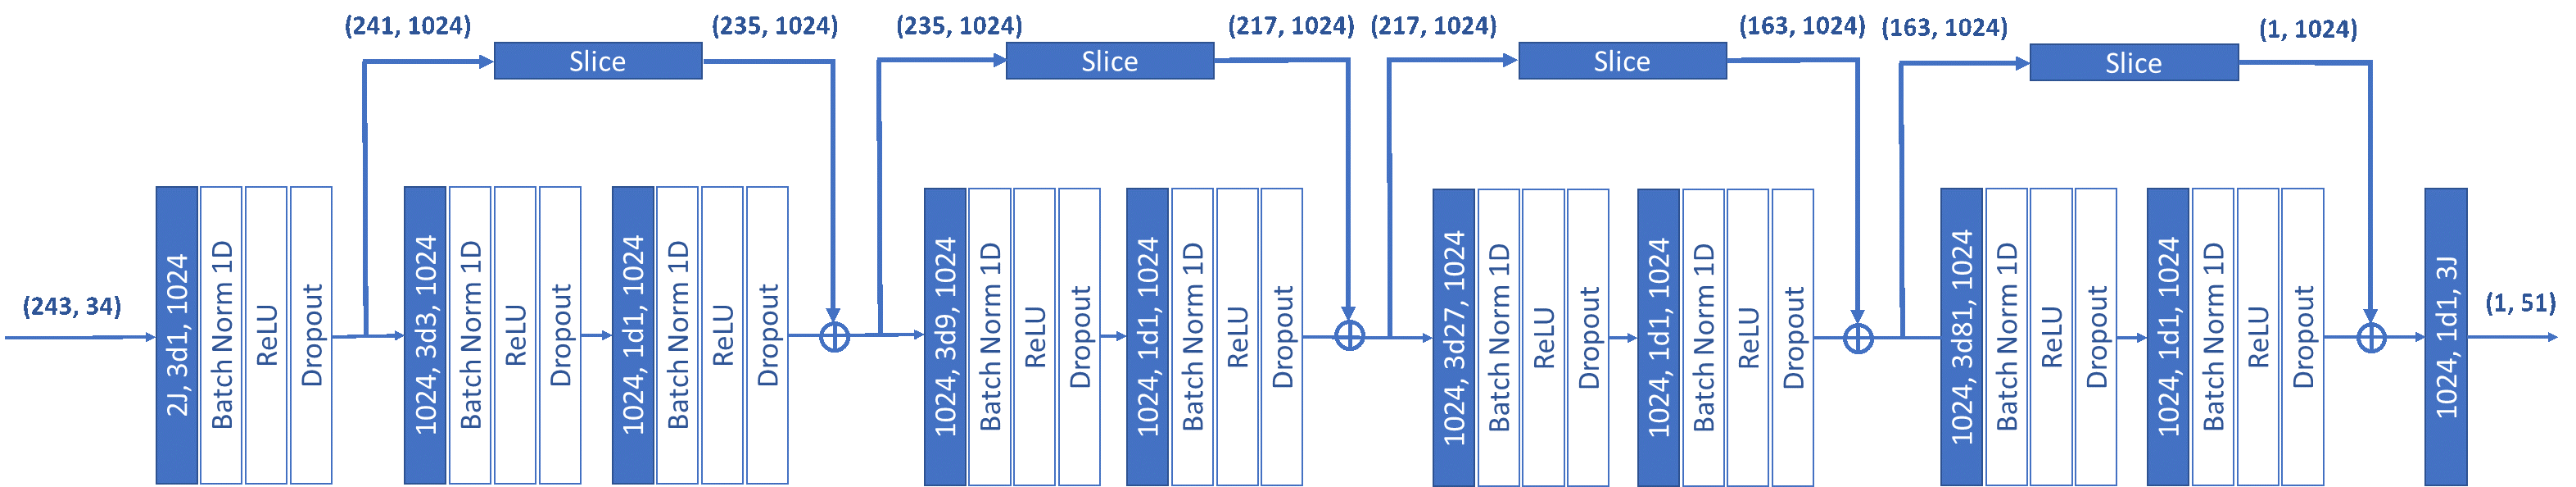
\includegraphics[scale=0.4]{figures/23.png}
	\caption{三维人体姿态估计模型网络结构}
	\label{fig:f23}
\end{figure}
在如上模型中每个残差块的感受野以W进行指数增加时,保证了参数的数量仅为线性增加。卷积核的大小W及空洞系数D使得感受野以树状覆盖所有的输入帧。最终网络输出所有帧的人体三维姿态。
\begin{figure}[h]
	\centering
	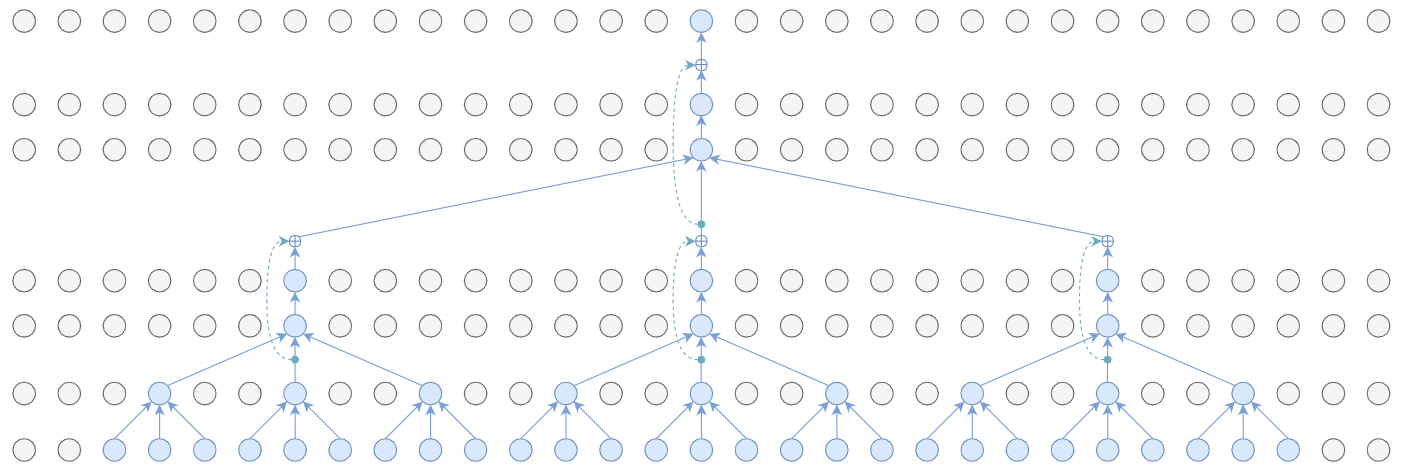
\includegraphics[scale=0.4]{figures/24.png}
	\caption{树状网络模型(W=3,B=3)}
	\label{fig:f24}
\end{figure}


\section{数据及实验}
\subsection{三维人体姿态数据集}{}
Human3.6M数据集具有360万个三维人体姿势和相应的图像,共11位实验者包括6位男性和5位女性,共有17个动作场景,诸如讨论、吃饭、运动、问候等动作。用4个严格校准的相机录制高分辨率的50Hz视频。并用高速运动动作捕捉系统提供准确的关节点三维位置,像素级的24个人体部位信息。同时严格控制背景元素,提供精准的人体位置边框。
HumanEva-I数据集包含用三个60赫兹的摄像机记录的经过校准的视频序列(4个灰度视频和3个RGB视频),与从运动捕捉系统获得的三维身体姿态同步。该数据库包含4名受试者执行6种常见动作(如散步、慢跑、打手势等)。给出了二维和三维姿态中计算误差的误差度量。该数据集包含训练、验证和测试集。本文采用15个关节点信息进行训练和测试。
PI-INF-3DHP 数据集,由 Max Planck Institute for Informatics 制作,是一个新发布的三维人体姿势数据集,包含 6 个7 个动作(背景为绿屏 (GS) 和无绿屏 (NoGS)),由动 (MoCap System)和 14 个 RGB 相机和 2 名受试者在室外的野外设置中执行动作。
由卡内基梅隆大学(CMU, Carnegie Mellon University)制作。使用了480个VGA摄像头,具有640 x 480的分辨率,视频帧率为25 fps,并使用了与其同步的31个HD摄像头,具有1920 x 1080分辨率,帧率为30 fps,在它们之间同步使用硬件时钟。同时,还使用了10个KinectⅡ传感器和5个DLP投影仪。采集了时长共5.5小时的65个视频序列,包含了150万个三维人体骨架信息。
在本文的工作中,选取Human3.6m数据集中的17个关节点信息,在(S1、S5、S6、S7、S8) 5个子集上进行训练,并用(S9、S11)2个子集作为测试集。

\subsection{实验结果}{}
本文使用评价指标为关节点平均坐标误差MPJPE (Mean Peer Joint Position Error),估计出的坐标与真实关节点坐标之间的欧氏距离。
本文采用Adam优化器,设置learning rate=0.001, decay=0.95,同时batch size=1024对Human3.6m数据集进行80 epoches的训练,训练及测试结果如下所示。
\begin{figure}[h]
	\centering
	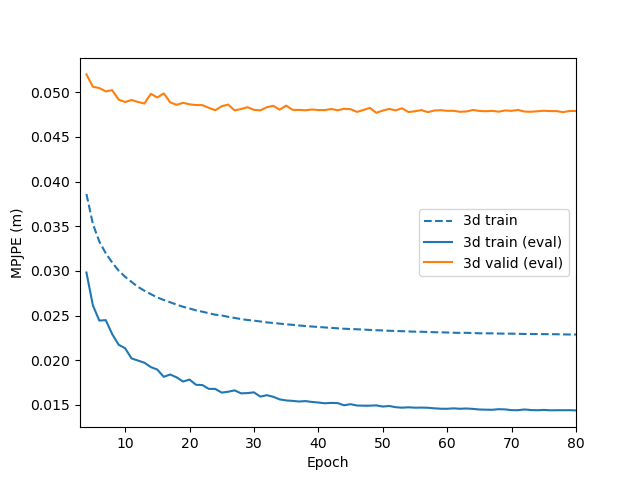
\includegraphics[scale=0.4]{figures/25.png}
	\caption{三维人体姿态估计模型MPJPE-Epoch曲线}
	\label{fig:f25}
\end{figure}
在针对Human3.6m数据集的姿态估计中,本文的方法可以流畅准确地还原出人体的三维动作,以该视频为例,本文的工作的输出结果与真实标注的差异如图x所示。可见估计结果中的三维姿态强依赖于二维关节点坐标,基本保证了三维姿态到相机坐标系的重投影与二维姿态一致。
\begin{figure}[h]
	\centering
	\includegraphics[scale=0.4]{figures/26.png}
	\caption{三维人体姿态估计结果对比真实标注(数据为Photo.54138969)}
	\label{fig:f26}
\end{figure}
%todo 插入videopose3d结果对比表格
        
\chapter{视频动作捕捉动画生成}
动作捕捉(MoCap, Motion Capture)是指利用多种传感器,如光感、惯性、摄像头等,来记录物体或人体运动过程中的动作的技术。在军事、影视、运动、医疗、机器人、计算机视觉及图形学等领域有着广泛且深入的应用。本章针对动作捕捉在电影制作、游戏开发等需要将动作绑定至角色模型制作三维动画的场景,利用深度学习人体姿态估计,对RGB单目单人视频中的人体动作进行提取,再绑定至角色模型,搭建低门槛、低成本、广泛场景的视频动作捕捉解决方案。

\section{整体框架}

视频动作捕捉动画生成的整体流程如图x所示,首先利用RGB摄像头,如手机摄像头,采集单人运动视频。第一步将视频送入第三章中的二维人体姿态估计模型对每一帧中的主要人物目标的各关节坐标进行估计。第二步将得到的二维坐标序列送入第四章的三维人体姿态估计模型进行三维坐标的估计。第三步,搭建人体骨骼模型,将三维坐标序列转换为描述骨骼运动的欧拉角序列,并写为bvh动作描述文件。第四步创建人体角色模型,利用动画生成软件将bvh文件描述的动作序列绑定至模型。最终生成三维动画,可在动画引擎中进行播放。
\begin{figure}[h]
	\centering
	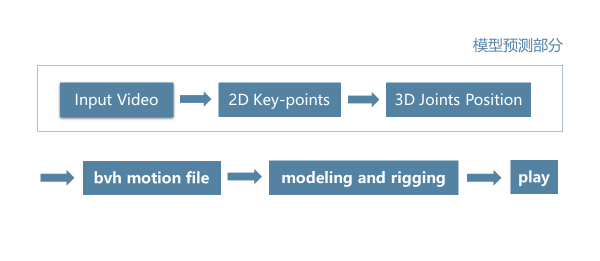
\includegraphics[scale=0.4]{figures/27.png}
	\caption{视频动作捕捉动画生成整体框架}
	\label{fig:f27}
\end{figure}

\section{实现细节}
\subsection{Bvh文件设计}{}
综合考虑人体姿态信息的多样性和复杂性,为了最大限度表达人体姿态,同时考虑数据量因素,现该领域研究人员一般用人体各个关键点来估人体姿态信息。基于骨骼关键点方法首次由  Johansson 在其经典的移动灯显示实验提出。人体姿态的大部分信息由主要的关节关键点即可描述。由此,人体姿态估计领域的研究大多基于该描述方法。目前主流的数据集的标签也采用标注骨骼关键点的方式。例如上述Human3.6m数据集中的人体骨骼关节点定义如图\ref{fig:f12}所示。在本文进行三维人体姿态估计时,以上人体骨骼模型也成为了由模型预测结果转为动作描述文件的基础。
由上一小节中对bvh文件的介绍可知,每个bvh文件描述一个运动目标,且运动目标由各个关节点构成,并以继承关系构建为骨骼树,具有唯一的父节点。故而对于本文所采集运动信息的人体目标,保留了21个人体关键关节点,设计并搭建了人体骨骼架构,具体的父子节点关系如下:

\begin{lstlisting}[language=python, label={lst:children}]
 self.children = {
    'Hip': ['RightHip', 'LeftHip', 'Spine'],
    'RightHip': ['RightKnee'],
    'RightKnee': ['RightAnkle'],
    'RightAnkle': ['RightAnkleEndSite'],
    'RightAnkleEndSite': [],
    'LeftHip': ['LeftKnee'],
    'LeftKnee': ['LeftAnkle'],
    'LeftAnkle': ['LeftAnkleEndSite'],
    'LeftAnkleEndSite': [],
    'Spine': ['Thorax'],
    'Thorax': ['Neck', 'LeftShoulder', 'RightShoulder'],
    'Neck': ['HeadEndSite'],
    'HeadEndSite': [],  # Head is an end site
    'LeftShoulder': ['LeftElbow'],
    'LeftElbow': ['LeftWrist'],
    'LeftWrist': ['LeftWristEndSite'],
    'LeftWristEndSite': [],
    'RightShoulder': ['RightElbow'],
    'RightElbow': ['RightWrist'],
    'RightWrist': ['RightWristEndSite'],
    'RightWristEndSite': []
}
\end{lstlisting}
进一步地,基于人体解剖学知识,将各个子关节相对于父关节的初始偏移方向定义如下:
\begin{lstlisting}[language=python, label={lst:direction}]
self.initial_directions = {
    'Hip': [0, 0, 0],
    'RightHip': [-1, 0, 0],
    'RightKnee': [0, 0, -1],
    'RightAnkle': [0, 0, -1],
    'RightAnkleEndSite': [0, -1, 0],
    'LeftHip': [1, 0, 0],
    'LeftKnee': [0, 0, -1],
    'LeftAnkle': [0, 0, -1],
    'LeftAnkleEndSite': [0, -1, 0],
    'Spine': [0, 0, 1],
    'Thorax': [0, 0, 1],
    'Neck': [0, 0, 1],
    'HeadEndSite': [0, 0, 1],
    'LeftShoulder': [1, 0, 0],
    'LeftElbow': [1, 0, 0],
    'LeftWrist': [1, 0, 0],
    'LeftWristEndSite': [1, 0, 0],
    'RightShoulder': [-1, 0, 0],
    'RightElbow': [-1, 0, 0],
    'RightWrist': [-1, 0, 0],
    'RightWristEndSite': [-1, 0, 0]
}
由此构成了人体骨骼模型的默认形态。
在人体解剖学中,骨骼的运动由关节运动主导,关节的运动与关节面形状贴合,而关节面形状也是在人体的长期活动中,肌肉作用下逐步获得、形成的,以上击力使得人体关节运动一般为绕某个轴进行的旋转运动。在上述简化的人体骨骼模型下,每个骨骼的旋转平面皆可由其他骨骼的方向定义,这为构造bvh文件数据部分的欧拉角任务提供了清晰明确、易于定义的旋转轴。故而针对根节点,即Hip节点保留3个Translation和3个Rotation共6个通道,其余子节点仅保留3个Ratation通道。生成的bvh文件样例附于附录。

\end{lstlisting}
\subsection{三维角色动作绑定}{}
在进行三维角色动画创作的过程中,当已经创建了一个骨骼结构的动作后,需要将动作与目标的实际模型进行捆绑,使得动作可以在目标模型上展示和播放,这个过程通常称为三维动画角色动作绑定或骨骼绑定(3D character rigging for animation)。
在本文的框架中,我们选择使用Autodesk的MotionBuilder软件,将上一小节生成的bvh文件与已有的人物模型进行绑定,MotionBuiler软件的图形工作界面如图\ref{fig:f28}所示。本文的工作利用其提供的Python借口进行动画的自动化生成。
\begin{figure}[h]
	\centering
	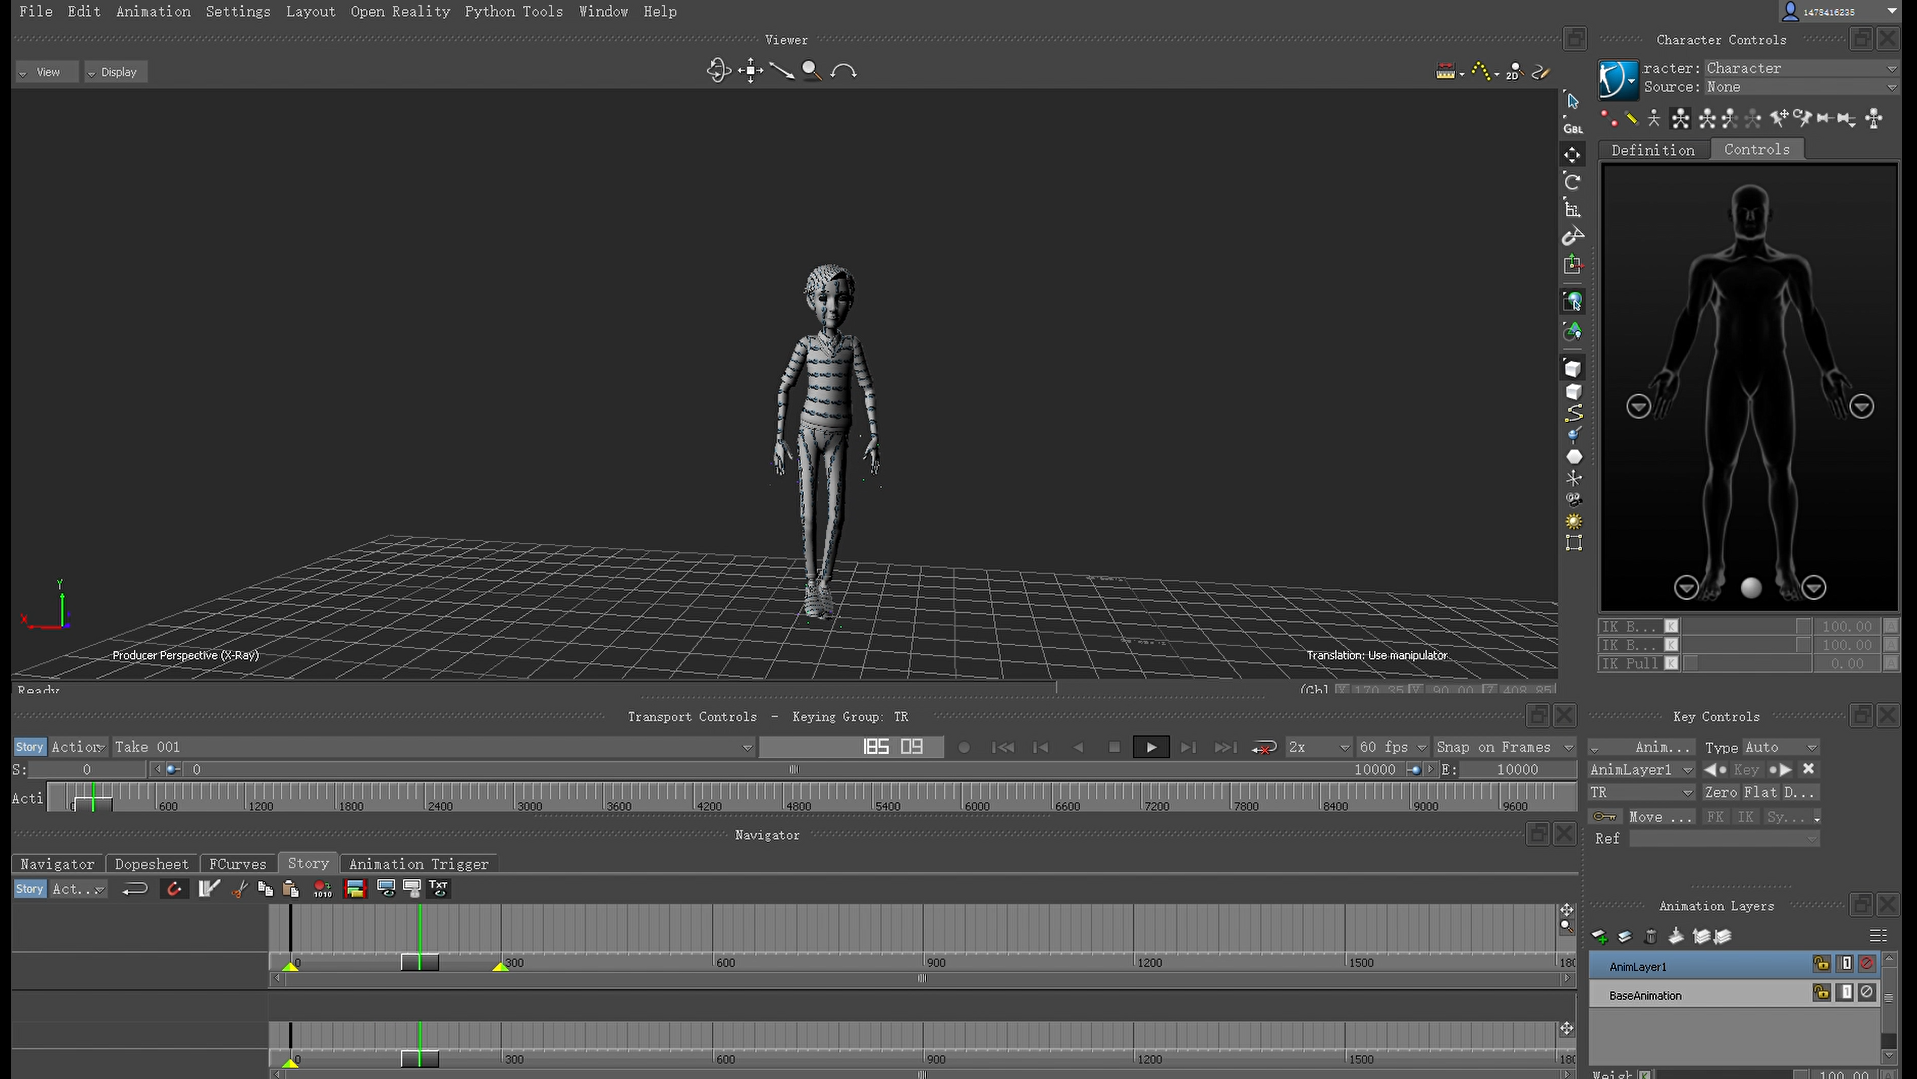
\includegraphics[scale=0.4]{figures/28.png}
	\caption{MotionBuilder图形工作界面}
	\label{fig:f28}
\end{figure}


\section{实现效果}
\subsection{人体姿态估计}{}
本文选取了网络视频,对其进行人体姿态估计结果如图\ref{fig:f29}所示。
\begin{figure}[h]
	\centering
	
\includegraphics[scale=0.4]{figures/XJTU_RED.png}
	\caption{自选视频的三维人体姿态估计结果}
	\label{fig:f29}
\end{figure}
在估计的过程中,三维姿态结果出现了偶然的不稳定情况,会出现突发的错误帧。在本文第四章中,指出了三维姿态结果对二维姿态结果的强依赖关系,本文针对此设计了对照实验,将我们的模型与将二维关节点真实坐标输入第四章模型输出的结果做了对比,如图\ref{fig:f30}所示。结果证明输出结果中出现的动作错乱的主要原因为二维关节点的识别和估计错误,可根据需要利用卡尔曼滤波进行平滑。
\begin{figure}[h]
	\centering
	\includegraphics[scale=0.4]{figures/30.png}
	\caption{输入为真实二维标注与二维估计模型预测结果的三维估计结果对比}
	\label{fig:f30}
\end{figure}

\subsection{动作绑定}{}
将上述模型对视频的预测结果,即三维关节点坐标转换为了关节旋转欧拉角,按照前述bvh文件设计生成了相应的bvh文件。在MotionBuilder软件中,对已有的人体角色模型进行了动作绑定,软件界面如图x,绑定结果如图x。

        
\chapter{总结与展望}
\echapter{Conclusions}

从项目的第一行代码写下到修复已知的最后一个bug且将项目暂时尘封,历时7个月。作为笔者本科阶段工作量最大的项目,它的工作并非简单地设计出工程架构、堆砌业务逻辑,还包括阅读理解大量Linux文档和已有开源库的实现。

\section{结论}{}

本文首先使用两步提升法对RGB单目单人视频分别进行了人体姿态序列的二维和三维的估计,并进一步搭建了一个完整的视频动作捕捉制作三维动画的框架。

% todo 可补充

在人体姿态估计任务方面,本文的工作可以对日常的人体姿态进行较为准确的还原,但目前的工作还具有以下局限性:
\begin{enumerate}
    \item 网络的泛化性不足。对快速的动作预测出的姿态速度较慢,对快速运动时不清晰帧的预测效果有限,对于非常见动作的预测准确性较差,在背景复杂时易出现混淆的情况。
    \item 网络对于上下文信息的提取能力有限。当对于多个三维姿态对应相同的二维姿态投影的歧义性发生时,易估计出反人体解剖学的三维姿态。
    \item 模型对于世界坐标系中人体根节点的位移的估计效果较差。
\end{enumerate}

在视频动作捕捉制作三维动画方面,本文的工作可以利用人体的动作制作出生动且还原度高的三维角色动画,但对于原始视频的采集仍具有以下要求:
\begin{enumerate}
    \item 固定相机位姿拍摄单人视频,保证人体部位全部入境。
    \item 目标人物距离与镜头的距离位于3到10米之间。
    \item 人物衣着简单,背景干净,避免遮挡与混淆。
\end{enumerate}

6.2 展望
针对如上问题,针对本文课题的未来工作仍然具有诸多挑战和极大的发展空间,也有诸多值得期待的改进方向:
\begin{enumerate}
    \item 在实际应用场景中,可以相应地丰富数据集,对不同距离,速度的动作进行全方面的采集。
    \item 人体姿态估计虽然具有着许多固有的难点,如投影歧义等。但人体本身的解剖学约束,以及人体动作中包含的丰富的语义信息以及上下文信息可以对姿态的估计提供高强度的帮助。可以利用如图卷积神经网络等模型,对如上深层信息进行进一步的提取。
    \item 视频动作捕捉的市场广阔,针对动作制作需求,可以对提取出的动作序列进行针对性的后处理优化,如消抖、平滑、清洗突变帧,稳定根节点位移,增强脚-地接触的重力效果等。
\end{enumerate}




    \xjtuendcontent

    % 将你要引用的文献的 BibTeX 放入 bibliography.bib
    \xjtubib{bibliography}

    %\xjtuappendix

        %% appendice.tex
%
% Aetf <aetf@unlimitedcodeworks.xyz>
% Copyright 2016 Aetf <aetf@unlimitedcodeworks.xyz>
%
% multiple1902 <multiple1902@gmail.com>
% Copyright 2011~2012, multiple1902 (Weisi Dai)
%
% Project Home: https://github.com/Aetf/xjtuthesis
%
% It is strongly recommended that you read documentations located at
%   https://github.com/Aetf/xjtuthesis/wiki
% in advance of your compilation if you have not read them before.
%
% This work may be distributed and/or modified under the
% conditions of the LaTeX Project Public License, either version 1.3
% of this license or (at your option) any later version.
% The latest version of this license is in
%   http://www.latex-project.org/lppl.txt
% and version 1.3 or later is part of all distributions of LaTeX
% version 2005/12/01 or later.
%
% This work has the LPPL maintenance status `maintained'.
%
% The Current Maintainer of this work is Aetf.
%
\xjtuappendixchapter{附录}

    \xjtuappendixsection{测试标题}

        The quick brown fox jumps over the lazy dog.

        \begin{figure}[h!]
          \centering
          
\includegraphics[width=6.67cm]{XJTU.pdf}
          \caption{西安交通大学}
          \label{fig:in-appendix}
        \end{figure}

        \xjtuappendixsubsection{三级标题}

            测试

            \xjtuappendixsubsubsection{四级标题}

                测试

\xjtuappendixchapter{还是附录}

    \xjtuappendixsection{测试}

        The quick brown fox jumps over the lazy dog.


    %\xjtuendappendix

    \xjtuspchapter{致谢}{致\qquad 谢}

        时光荏苒,大学生涯即将画上句点,回顾在西安交通大学少年班的六年经历,我迷茫过,挫败过,也重新拾起过勇气,带着希望和坚强前进过。在这条成长之路上,我获得过许多来自家人、老师、朋友的帮助和支持,在此向他们表示由衷的感谢。

首先感谢我的父母,他们为我的成长提供了一个包容,富足,充满爱的环境。他们的呵护与支持使得我无论在怎样的困境下,都可以永远热爱生活,积极对待生命。

感谢魏平老师在我毕业设计的工作期间给我提供了正确的方向和细致的指导,魏平老师扎实的专业素养、严谨深刻的学术风格和充满耐心的交流方式令我获益匪浅。

感谢北京大学人工智能创新中心,感谢雷鸣老师、张金娜老师以及AIIC的同学们,在这一年中给予了我辅导和技术资源支持,成为了我研究生生涯的领路人。愿我们在未来的学习生涯中能并肩作战,结成牢固的友谊,收获属于每个人的成长。

感谢西安交通大学的学长学姐,计算机系的同学们,以及我可爱的舍友们,我们曾一起在舞台上歌唱舞蹈,一起在球场上挥洒汗水,一起为了同一个目标奋不顾身,无数个奖状上都曾共同出现过我们的名字,无数个深夜都曾在星空下一起欢笑。在保研推免期间,尽管我们散布在天涯海角,你们仍给予了我至关重要的帮助与及时的支持,愿我们能携手出发,在未来奔向各自的辉煌的旅程。

感谢王晓芙和宋晓彤,与我在2011年相识,如今我们即将相伴十载,在我最迷茫的时候,你们曾是我与外面的世界唯一的连结,是我永远的精神支柱。愿我们终能像六年前所期盼的那样,仗剑天涯,道一句青春不朽。

最后,感谢西安交通大学2015级少年班,这是一个丰富、独特、有灵气的集体,在这里成长的六年是我人生中的最富有色彩的一笔。在这里,青涩与成熟在碰撞,现实与理想在碰撞,挫折与希望在碰撞,青春与成长在碰撞,每一次碰撞都能迸发出闪耀的火花,映照出少年的模样。我聆听过恶魔的低语,也感受到过天使的光明。从来到走,一束温暖的光洒在了我前进的路上。它照亮了未来,消散了过去,驱赶了恐惧,让勇敢与坚强从泥土深处生长,开出另一种完整,也愿它永远灿烂。

待来日,相逢意气为君饮,系马高楼垂柳边。


\end{document}

